\documentclass[11pt,a4paper]{article}
\usepackage[T1]{fontenc}
\usepackage{lmodern}
\usepackage[margin=22mm,headheight=14pt]{geometry}
\usepackage{amsmath,amssymb,bm,booktabs,tabularx,array,graphicx}
\usepackage[dvipsnames]{xcolor}
\usepackage{enumitem,fancyhdr,microtype}
\usepackage{float}
\usepackage[colorlinks=true,linkcolor=MidnightBlue,urlcolor=MidnightBlue,citecolor=MidnightBlue]{hyperref}
\usepackage[most]{tcolorbox}
\definecolor{ink}{HTML}{193B60}
\tcbset{colback=ink!4,colframe=ink!65,boxrule=0.6pt,arc=1mm,left=2mm,right=2mm,top=1.2mm,bottom=1.2mm}
\setlength{\parindent}{0pt}
\setlength{\parskip}{6pt}
\setlist{nosep,leftmargin=5mm}
\renewcommand{\arraystretch}{1.18}
\pagestyle{fancy}
\fancyhf{}
\fancyhead[L]{\small QFT Project B | Step 1}
\fancyhead[R]{\small Group B}
\fancyfoot[C]{\thepage}
\newcommand{\dd}{\mathrm{d}}
\newcommand{\ProjectTitle}{What Quantum Trace Can a Heavy Particle Leave?}
% Generated by code/step1.py. Do not edit by hand.
\newcommand{\ReferenceRatio}{0.035}
\newcommand{\DerivativeError}{1.053\times 10^{-9}}
\newcommand{\DilationError}{3.886\times 10^{-12}}
\newcommand{\PassedChecks}{10}
\newcommand{\PythonVersion}{3.12.14}
\newcommand{\NumpyVersion}{2.3.5}
\newcommand{\MatplotlibVersion}{3.10.8}

\newcommand{\ConvergenceRows}{%
$1.000\times 10^{-2}$ & $1.028\times 10^{-3}$ \\
$5.000\times 10^{-3}$ & $2.569\times 10^{-4}$ \\
$2.500\times 10^{-3}$ & $6.423\times 10^{-5}$ \\
$1.250\times 10^{-3}$ & $1.606\times 10^{-5}$ \\
$1.000\times 10^{-4}$ & $1.028\times 10^{-7}$ \\
$1.000\times 10^{-5}$ & $1.053\times 10^{-9}$ \\
}

\newcommand{\RepositoryLine}{%
\href{https://github.com/rawatpriyansh17/QFT-PROJECT-GROUP-B/tree/main/step1}{Step 1 code folder}.\\[2mm]
\href{https://github.com/rawatpriyansh17/QFT-PROJECT-GROUP-B/blob/main/step1/step1.py}{Python script}\quad
\href{https://github.com/rawatpriyansh17/QFT-PROJECT-GROUP-B/blob/main/step1/config.json}{Configuration}\quad
\href{https://github.com/rawatpriyansh17/QFT-PROJECT-GROUP-B/blob/main/step1/requirements.txt}{Dependencies}\quad
\href{https://github.com/rawatpriyansh17/QFT-PROJECT-GROUP-B/blob/main/step1/README.md}{Run instructions}.\\[2mm]
\href{https://github.com/rawatpriyansh17/QFT-PROJECT-GROUP-B/tree/main/step1/results}{Numerical results}\quad
\href{https://github.com/rawatpriyansh17/QFT-PROJECT-GROUP-B/tree/main/step1/figures}{Figures}\quad
\href{https://github.com/rawatpriyansh17/QFT-PROJECT-GROUP-B/blob/main/step1/results/summary.json}{Validation summary}.\\[2mm]
Code and outputs: \href{https://github.com/rawatpriyansh17/QFT-PROJECT-GROUP-B/commit/28ea4789ee74f91254664afeb9e5b23da096f1a5}{\texttt{28ea478}}.}

\hypersetup{pdftitle={QFT Project B - Step 1: Spacetime, Fields and Observables},pdfauthor={Priyansh Rawat, Mayank Sinha, Samarth Bhatnagar}}

\begin{document}
\hypersetup{pageanchor=false}
\begin{titlepage}
\centering
\vspace*{2mm}

\includegraphics[width=36mm]{assets/bits_logo.png}\par
\vspace{13mm}
{\Large\bfseries BITS PILANI K.K. BIRLA GOA CAMPUS\par}
\vspace{3mm}
{\large\bfseries Department of Physics\par}
\vspace{19mm}
{\LARGE\bfseries What Quantum Trace Can\\[2mm] a Heavy Particle Leave?\par}
\vspace{5mm}
{\large Curvature--Spectator Entanglement\\ and the Cosmological Collider\par}
\vspace{8mm}
{\large\bfseries Step 1: Spacetime, Fields and Observables\par}
\vspace{17mm}
{\Large\bfseries Group-B\par}
\vspace{4mm}
\begin{tabular}{ll}
Priyansh Rawat & 2023B5A70968G\\
Mayank Sinha & 2023B5A70942G\\
Samarth Bhatnagar & 2023B5A70853G
\end{tabular}
\vfill
{\large Under Professor: Rudranil Basu\par}
\vspace{7mm}
{19 October 2026\par}
\vspace{5mm}
\end{titlepage}
\setcounter{page}{1}
\hypersetup{pageanchor=true}

\section{Objective and spacetime convention}
\textbf{Project question.} How does light--spectator entanglement depend on mass and mixing, and does more entanglement imply a stronger heavy-field three-point signal? Quadratic mixing can produce Gaussian entanglement; a connected three-point signal also needs a non-Gaussian interaction.

\textbf{Scope.} We fix the background, action, normalisation and observables, then derive and check the specified single-field squeezed reference. Coupled-field entropy and the spectator bispectrum belong to later steps.

\subsection{Expansion and horizon crossing}
We use natural units $\hbar=c=1$ and an exact de Sitter calculational background,
\begin{equation}
\dd s^2=a^2(\eta)(-\dd\eta^2+\dd\bm{x}^2),\qquad
a(\eta)=-\frac{1}{H\eta},\qquad \eta<0,\quad H>0.
\label{eq:background}
\end{equation}
Here $H$ is constant, $\eta$ is conformal time and $a$ is the scale factor. Conformal time and cosmic time obey $\dd t=a\,\dd\eta$. Differentiation with respect to $\eta$ is denoted by a prime. As $\eta$ increases towards zero, $a$ grows.

For a fixed comoving wavenumber $k=|\bm{k}|>0$, define
\begin{equation}
\boxed{x=-k\eta=\frac{k}{aH}.}
\label{eq:x}
\end{equation}
The physical wavenumber is $k/a$, so $x$ compares it with the expansion rate. Evolution proceeds from large to small $x$. The numerical convention is $H=1$, with masses and mixing restored using ratios to $H$.

\begin{center}
\begin{tabular}{lll}
\toprule
Regime & Condition & Interpretation\\
\midrule
Inside the horizon & $x\gg1$ & Physical wavelength is much shorter than $H^{-1}$.\\
Horizon crossing & $x=1$ & $k=aH$, with $a_*=k/H$.\\
Outside the horizon & $x\ll1$ & Physical wavelength is much longer than $H^{-1}$.\\
\bottomrule
\end{tabular}
\end{center}
Here the usual horizon convention compares $a/k$ with $H^{-1}$; retaining a literal wavelength $2\pi a/k$ introduces the corresponding factor of $2\pi$.
\begin{figure}[H]
\centering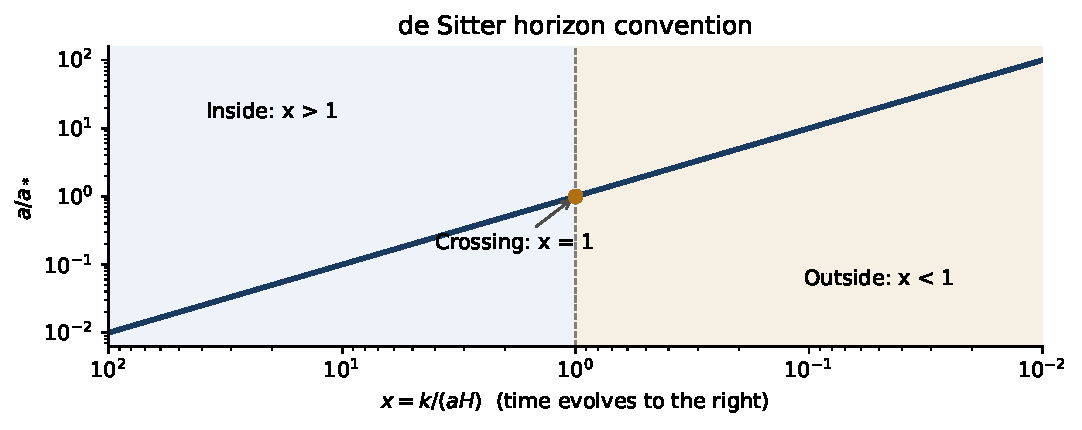
\includegraphics[width=0.78\linewidth]{figures/horizon_map.pdf}
\caption{For $H=k=1$, $a/a_*=1/x$. The axis follows forward time. This checks the background convention, not field-mode evolution.}
\end{figure}

\newpage
\section{Fields, action and physical parameters}
We use the quadratic action
\begin{align}
S_2=\int\dd\eta\,\dd^3x\,\Bigg\{&\frac{a^2}{2}
\left[(q')^2-(\bm{\nabla}q)^2+(\sigma')^2-(\bm{\nabla}\sigma)^2\right]\nonumber\\
&-\frac{a^4m^2}{2}\sigma^2+a^3\rho\,q'\sigma\Bigg\}.
\label{eq:action}
\end{align}
\begin{center}
\begin{tabularx}{\linewidth}{lX}
\toprule
Symbol & Meaning\\
\midrule
$q$ & Light scalar perturbation, proportional to the curvature perturbation at linear order.\\
$\sigma$ & Spectator scalar field; it is the additional degree of freedom to be traced out when studying the light subsystem.\\
$m$ & Spectator mass parameter in the quadratic action.\\
$\rho$ & Constant derivative-mixing strength multiplying $q'\sigma$.\\
$M=m/H$ & Dimensionless mass, used when comparing masses with the expansion rate.\\
$g=\rho/H$ & Dimensionless mixing strength.\\
\bottomrule
\end{tabularx}
\end{center}

\subsection{Reading the action}
The terms containing time derivatives are kinetic terms. The gradient terms describe spatial variation, and the $m^2\sigma^2$ term supplies the spectator mass. The last term couples the time variation of $q$ to $\sigma$. Thus, at nonzero $\rho$, the two fields do not evolve independently. At $\rho=0$ the quadratic action separates into a massless light field and a massive spectator.

The mixing contains a derivative. Consequently, the momentum conjugate to $q$ must eventually be obtained from $\partial\mathcal L/\partial q'$, rather than assumed to be $a^2q'$. The Legendre transform and canonical evolution are the subject of Step 3; here we retain the action without expanding or dropping any terms.

\subsection{Dimensions and normalisation}
With dimensionless $a$ and coordinates of inverse-mass dimension, the action is dimensionless when
\begin{equation}
[q]=[\sigma]=[H]=[m]=[\rho]=\text{mass},\qquad [M]=[g]=1.
\end{equation}
For example, $[q']=\text{mass}^2$ and $[\rho q'\sigma]=\text{mass}^4$, matching the kinetic and mass terms. The integration measure has dimension $\text{mass}^{-4}$.

Write the linear curvature conversion as $q=C\zeta$, where $\zeta$ is dimensionless and $C$ has mass dimension one. The guide does not fix a numerical value for $C$. We therefore keep $q$ and $\zeta$ observables distinct and do not equate their reduced bispectra. A conversion to a specific inflationary model would require its stated background normalisation.

\begin{tcolorbox}
\textbf{Approximation fixed for the project.} The core calculation uses the specified two-field model on de Sitter space. It does not require the full gravitational cubic action. Later, Gaussian entropy will be calculated within the quadratic theory, while the spectator bispectrum will be evaluated to leading order in a separately specified cubic coupling.
\end{tcolorbox}

\newpage
\section{Fourier convention and observables}
We use the following Fourier convention for both fields:
\begin{equation}
q(\eta,\bm{x})=\int\frac{\dd^3k}{(2\pi)^3}\,q_{\bm{k}}(\eta)e^{i\bm{k}\cdot\bm{x}},
\qquad [a_{\bm{k}},a^\dagger_{\bm{p}}]=(2\pi)^3\delta^3(\bm{k}-\bm{p}).
\label{eq:fourier}
\end{equation}
For a real field, $q_{-\bm{k}}=q_{\bm{k}}^\dagger$. Opposite momenta therefore obey a reality condition; they are not two independent real oscillators. The cosine/sine sector counting needed for entropy will be fixed in Step 2.

Translation invariance gives the momentum-conserving delta functions:
\begin{align}
\langle q_{\bm{k}}q_{\bm{p}}\rangle
&=(2\pi)^3\delta^3(\bm{k}+\bm{p})P_q(k),\label{eq:power}\\
\langle q_{\bm{k}_1}q_{\bm{k}_2}q_{\bm{k}_3}\rangle_c
&=(2\pi)^3\delta^3(\bm{k}_1+\bm{k}_2+\bm{k}_3)
B_q(k_1,k_2,k_3).\label{eq:bispectrum}
\end{align}
$P_q$ is the power spectrum. $B_q$ is the connected bispectrum, measuring a three-point correlation after disconnected contributions are removed. Momentum conservation requires the three vectors to close into a triangle. A squeezed triangle has $k_L\ll k_S$, with two nearly equal short-wavelength sides.

\subsection{Power spectrum versus dimensionless power}
For the curvature perturbation, define
\begin{equation}
\Delta_\zeta^2(k)=\frac{k^3}{2\pi^2}P_\zeta(k),\qquad
n_s-1=\frac{\dd\ln\Delta_\zeta^2}{\dd\ln k}.
\label{eq:tilt}
\end{equation}
For constant $n_s$, $\Delta_\zeta^2\propto k^{n_s-1}$, so
\begin{equation}
P_\zeta(k)\propto k^{n_s-4}.
\label{eq:powerlaw}
\end{equation}
The exponent of $P_\zeta$ is therefore $n_s-4$, rather than $n_s-1$. Mixing these two spectra would give the wrong squeezed-limit coefficient.

\subsection{Keeping the field conversion explicit}
At a common evaluation time, a scale-independent conversion $q=C\zeta$ gives
\begin{equation}
P_q=C^2P_\zeta,\qquad B_q=C^3B_\zeta,\qquad
\frac{B_\zeta}{P_\zeta(k_L)P_\zeta(k_S)}
=C\,\frac{B_q}{P_q(k_L)P_q(k_S)}.
\end{equation}
In this Fourier convention, $[P_q]=\text{mass}^{-1}$ and $[B_q]=\text{mass}^{-3}$, whereas $[P_\zeta]=\text{mass}^{-3}$ and $[B_\zeta]=\text{mass}^{-6}$. A useful later dimensionless spectator quantity is $H B_q/(P_qP_q)$, for the later spectator calculation. It equals the curvature ratio only if the conversion factor is $C=H$.

\textbf{Gaussian baseline.} For a centred Gaussian state evolved with the quadratic action, the connected three-point function vanishes. This can coexist with nonzero light--spectator entanglement. The value derived next is a separate single-clock curvature reference, rather than a bispectrum generated by Eq.~\eqref{eq:action} alone.

\newpage
\section{Derivation of the single-field squeezed reference}
In the single-clock attractor setting, a sufficiently long curvature mode is approximately constant across a short-scale region. Its leading effect can be represented by a spatial dilation. The short-scale spectrum conditioned on a small long mode $\zeta_L$ transforms as~\cite{maldacena,creminelli}
\begin{equation}
P_\zeta(k\mid\zeta_L)=e^{-3\zeta_L}P_\zeta(ke^{-\zeta_L}).
\label{eq:dilation}
\end{equation}
The argument changes because the local spatial scale changes. The prefactor accounts for the three-dimensional Fourier volume. Expanding both factors to first order gives
\begin{align}
e^{-3\zeta_L}&=1-3\zeta_L+O(\zeta_L^2),\\
P_\zeta(ke^{-\zeta_L})&=P_\zeta(k)-\zeta_L k\partial_kP_\zeta(k)+O(\zeta_L^2),\\
\delta P_\zeta(k)&=-\zeta_L(3+k\partial_k)P_\zeta(k)+O(\zeta_L^2).
\label{eq:delta}
\end{align}
Correlating this modulation with the long mode supplies its power spectrum. With the overall momentum delta function removed,
\begin{equation}
\lim_{k_L/k_S\to0}B_\zeta(k_L,k_S,k_S)
=-P_\zeta(k_L)(3+k_S\partial_{k_S})P_\zeta(k_S).
\label{eq:consistency}
\end{equation}
Now insert $P_\zeta(k)=A_0k^{n_s-4}$, with $A_0$ independent of $k$:
\begin{align}
k\partial_kP_\zeta(k)&=(n_s-4)P_\zeta(k),\\
(3+k\partial_k)P_\zeta(k)&=[3+n_s-4]P_\zeta(k)
=(n_s-1)P_\zeta(k).
\end{align}
Dividing Eq.~\eqref{eq:consistency} by the two power spectra yields the required result:
\begin{tcolorbox}
\begin{equation}
\boxed{\lim_{k_L/k_S\to0}
\frac{B_\zeta(k_L,k_S,k_S)}{P_\zeta(k_L)P_\zeta(k_S)}
=-(n_s-1)=1-n_s=\ReferenceRatio\quad(n_s=0.965).}
\end{equation}
\end{tcolorbox}
The ratio is positive for the specified red tilt. At $n_s=1$ it vanishes, providing a useful control. The number $0.035$ is this particular dimensionless ratio; it is not the unnormalised bispectrum or a direct estimate of a spectator mass.

\subsection{Applicability of the reference}
This argument uses a long adiabatic mode that acts as a dilation in the single-clock attractor regime. It is not a claim that all multifield or non-attractor models obey the same relation. We use this reference to compare with the extra spectator contribution.

The prescribed $n_s=0.965$ is an external reference input. It is not derived from the massless field on the exact de Sitter background in Eq.~\eqref{eq:background}. In particular, we do not add $0.035$ to a later spectator bispectrum calculated in the model.

\newpage
\section{Reproducible numerical validation}
The accompanying Python script implements two numerical checks of the analytic coefficient. For an arbitrary positive amplitude $A$ and pivot $k_*$, it uses
\begin{equation}
P_\zeta(k)=\frac{A}{k^3}\left(\frac{k}{k_*}\right)^{n_s-1}.
\end{equation}
The normalisation is illustrative; no observational amplitude is fitted. The script evaluates 121 logarithmically spaced values with $10^{-3}\leq k/k_*\leq10^3$, using $A=k_*=1$.

\textbf{Check 1: differentiate the power directly.} With fractional step $h$,
\begin{equation}
R_h(k)=-3-\frac{P_\zeta(k(1+h))-P_\zeta(k(1-h))}{2hP_\zeta(k)}.
\end{equation}
The central difference has an $O(h^2)$ truncation error. Refinement gives:
\begin{center}
\begin{tabular}{cc}
\toprule Fractional step $h$ & $\max_k|R_h-(1-n_s)|$\\\midrule
\ConvergenceRows
\bottomrule
\end{tabular}
\end{center}
\textbf{Check 2: differentiate the finite dilation.} Define $P(k\mid\epsilon)$ using Eq.~\eqref{eq:dilation} and compute
\begin{equation}
R_\epsilon(k)=\frac{P_\zeta(k\mid\epsilon)-P_\zeta(k\mid-\epsilon)}{2\epsilon P_\zeta(k)}.
\end{equation}
At $h=10^{-5}$ and $\epsilon=10^{-4}$, the maximum absolute errors are $\DerivativeError$ and $\DilationError$, respectively. Both are below the configured absolute tolerance $5\times10^{-8}$. These are numerical differentiation errors in a known benchmark, not uncertainties on a measured cosmological signal.
\begin{figure}[H]
\centering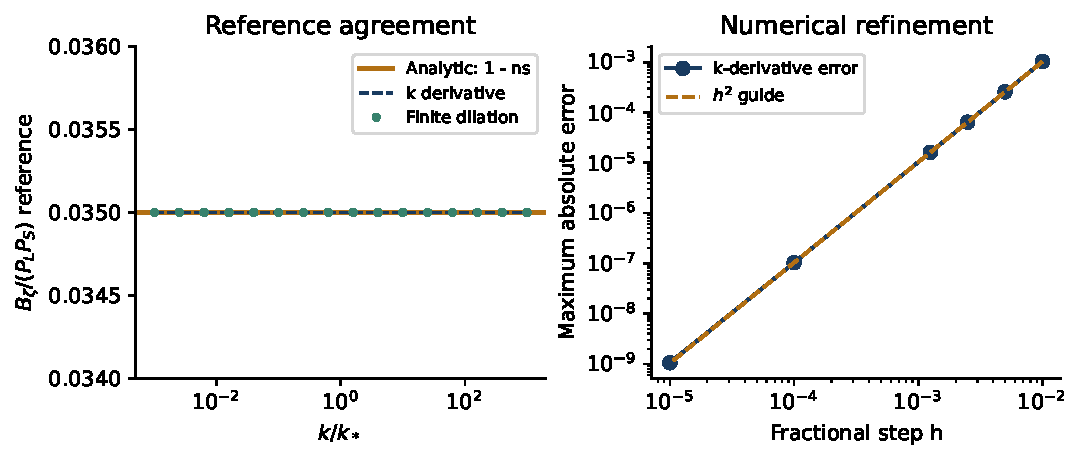
\includegraphics[width=\linewidth]{figures/reference_validation.pdf}
\caption{Left: the analytic value $0.035$ agrees with both numerical routes over six decades of $k$. Right: direct differentiation improves approximately as $h^2$. The calculations check the response identity; they do not evaluate a finite-squeezing or spectator bispectrum.}
\end{figure}

\newpage
\section{Results, reproducibility and next step}
\subsection{Validation outcome}
All \PassedChecks{} configured checks passed. In addition to the two derivative routes, the script checks the $n_s=1$ zero reference, red- and blue-tilt controls, cancellation of the arbitrary amplitude and pivot, second-order refinement, and the horizon identity $x=k/(aH)$. These tests verify different features of the implementation, though both derivative routes share the same input power spectrum; they are not two independent physical predictions.

\textbf{Established in Step 1.} The background, Fourier convention, dimensions, action and observable normalisations are fixed. The required squeezed reference is $0.035$ at $n_s=0.965$, with numerical checks supporting the algebra. No entropy map, coupled-field power spectrum, heavy-field frequency or mass estimate is claimed at this stage.

\subsection{Code and reproduction}
The implementation is organised in a \texttt{step1/} folder. From the repository root, run:
\begin{quote}\small\ttfamily
python3 -m pip install -r step1/requirements.txt\\
python3 step1/step1.py --config step1/config.json
\end{quote}
The two supporting data tables and validation summary are included in \texttt{step1/results/}, with PNG previews in \texttt{step1/figures/}. The README explains each figure and table. Running the script regenerates these outputs and vector PDFs for report preparation. Inputs are in \texttt{config.json}; the summary records checks, software versions and code/configuration hashes.

The calculation used Python \PythonVersion{}, NumPy \NumpyVersion{} and Matplotlib \MatplotlibVersion{}. It is deterministic and uses no random sampling.

\textbf{Code availability.} \RepositoryLine

\subsection{Immediate next step}
Step 2 will first validate Gaussian entropy for two ordinary coupled oscillators. It will reproduce the assigned $\nu=0.502816542$ and $s=0.0193599304$ benchmark, test zero coupling, increase the coupling to $0.6$, and check invariance under a local canonical rescaling. Entropy will be reported in nats per real sector, with the nonzero $\pm\bm{k}$ pair carrying twice that value. Subsequent steps will derive canonical equations before evolving cosmological modes.


\begin{thebibliography}{9}\small
\bibitem{maldacena} J.~Maldacena, \emph{Non-Gaussian features of primordial fluctuations in single field inflationary models}, JHEP 05 (2003) 013. \href{https://arxiv.org/abs/astro-ph/0210603}{arXiv:astro-ph/0210603}.
\bibitem{creminelli} P.~Creminelli and M.~Zaldarriaga, \emph{Single field consistency relation for the 3-point function}, JCAP 10 (2004) 006. \href{https://arxiv.org/abs/astro-ph/0407059}{arXiv:astro-ph/0407059}.
\end{thebibliography}

\newpage
\section{Contributions}
\begin{center}
\begin{tabularx}{\linewidth}{p{34mm}X}
\toprule
Member & Contribution\\\midrule
Priyansh Rawat & Physical setting, quadratic action and shared conventions; review of numerical checks and interpretation.\\[3mm]
Samarth Bhatnagar & Fourier conventions, dimensional analysis and the $q$--$\zeta$ conversion; review of the squeezed-limit derivation.\\[3mm]
Mayank Sinha & Numerical implementation, validation, data and figures; reproduction instructions and report consistency.\\
\bottomrule
\end{tabularx}
\end{center}
\end{document}
